\begin{figure}[H]
\centering
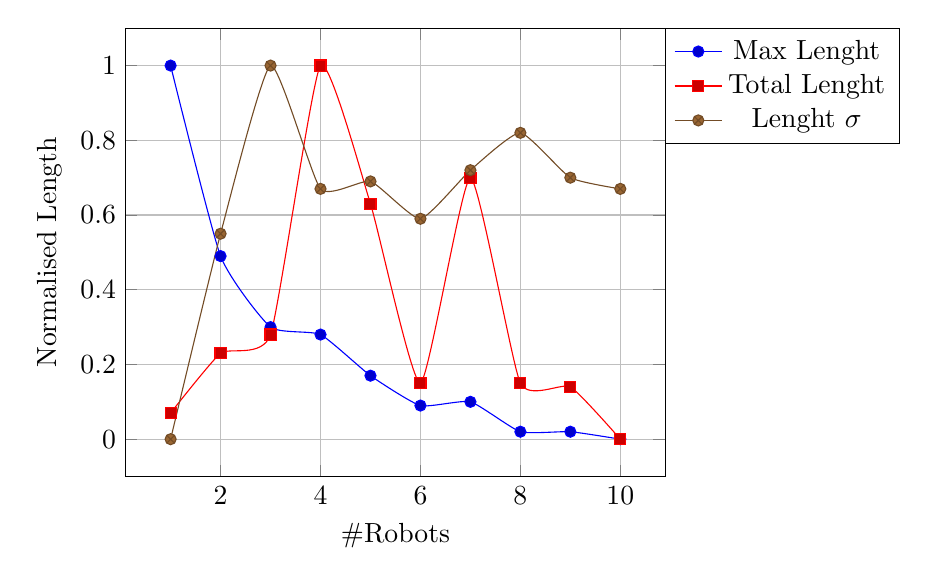
\begin{tikzpicture}
	\begin{axis}[
%		height=9cm,
%		width=9cm,
		grid=major,
                legend style = {at={(1,1)}, anchor=north west},
		xlabel=\#Robots,
		ylabel=Normalised Length,
		smooth,
		tension=0.3
	]

	\addplot coordinates {
(1, 1.00)
(2, 0.49)
(3, 0.30)
(4, 0.28)
(5, 0.17)
(6, 0.09)
(7, 0.10)
(8, 0.02)
(9, 0.02)
(10, 0.00)
	};
	\addlegendentry{Max Lenght}

	\addplot coordinates {
(1, 0.07)
(2, 0.23)
(3, 0.28)
(4, 1.00)
(5, 0.63)
(6, 0.15)
(7, 0.70)
(8, 0.15)
(9, 0.14)
(10, 0.00)
	};
	\addlegendentry{Total Lenght}

	\addplot coordinates {
(1, 0.00)
(2, 0.55)
(3, 1.00)
(4, 0.67)
(5, 0.69)
(6, 0.59)
(7, 0.72)
(8, 0.82)
(9, 0.70)
(10, 0.67)
	};
	\addlegendentry{Lenght $\sigma$}
	\end{axis}
\end{tikzpicture}
\caption{Variation of the performance indexes increasing the number of robots, for the 15x15 grid using the Node Counting algorithm}
\end{figure}